\chapter{Introduction}
    计算机视觉给予计算机顶尖猎杀者的通行证(眼睛).
    
    这门课重点在三维重建

    规范:网上的东西都引用一下为好

    \section{What is Computer Vision}

    \subsection{A standard computer vision system }

    摄像机(Camera) 照一个有 光源(Lighting) 的 场景(Scene) 通过 视觉算法(Vision Software) 转换为 场景描述(Scene Description).
    
    识别场景中属性
    \begin{enumerate}
        \item 3D形状
        \item 辨识物体
        \item 发生事件
    \end{enumerate}

    \subsection{Computer vision tasks}

    \begin{enumerate}
        \item Reconstruction(三维重建)
        \item Understanding(图像理解)
        \item Synthesis(图像合成)
    \end{enumerate}
    \subsection{Why is computer vision hard}
    计算机所视为一个矩阵(所以线性代数特别多),需要从数字中提取信息.

    人工智能现阶段瓶颈在我们对人脑认识并不清晰.视觉是个基本功能,但我们未知其如何具体实现的.计算机与人类各有优劣,需要探寻其不同的具体实现方式.

    如何把问题转换成数学问题.

    \subsection{Human perception}
    Shortcomings\&一些视错觉:明暗分辨,光流,人对三维旋转的感知需要深度(eg:遮挡关系).

    Advantages:理解与想象的能力,可以从较少信息的图像获取较多的信息.
    \section{What is Vision Used For}
    \subsection{Applications}
    \begin{enumerate}
        \item 人脸识别:点云(3D信息,安全),红外
        \item \transtip{DeepFake}{AI换脸}:危险.jpg,开源但被下了.
        \item \transtip{Augmented reality}{现实增强}:美颜,特效(确定关键点来改变) eg:mediapipe(开源)
        \item \transtip{Factory Automation,Vision Inspection}{工业检测}
        \item \transtip{Optical Character Recognition(OCR)}{光学文字识别}
        \item \transtip{Video Surveillance}{监控}
        \item \transtip{Human Computer Interaction}{人机交互}:\transtip{Optical Mouse}{光学鼠标},\transtip{Motion Sensing Games}{体感游戏}(识别骨架),\transtip{Motion Capture}{动作捕捉}
        \item \transtip{Digital Human}{数字人}:三维建模,动作捕捉
        \item \transtip{Sports Broadcasting}{体育分析}
        \item \transtip{3D Street View}{3D街景}:以前做不到,但现在可以真3D街景了
        \item VR Tour
        \item \transtip{Visual Localization and Navigation}{视觉导航}:用视觉定位.
        \item \transtip{Autonomous Navigation}{自动导航}:视觉定位
        \item \transtip{Robot Perception}{机器人感知}
        \item \transtip{Autonomous Driving}{自动驾驶}
        \item \transtip{Free Viewpoint Video}{全息呈现}
        \item \transtip{Medical Image Analysis}{医学影像分析}
    \end{enumerate}
    \subsection{Vision research}
    计算机视觉三大顶级会议:CVPR,ICCV,ECCV

    图形学顶会:ACM\_SIGGRAPG
    \section{Course Overview}
    \subsection{Target}
    进入这个领域, 用数学描述以解决问题(线性代数与优化).PS:Lab很硬
    \subsection{Overview}
    \begin{enumerate}
        \item Basic.(Lec.02 - Lec.04)
        \begin{enumerate}
            \item Lec.02: \transtip{图像形成}{Image formation}
            \begin{enumerate}
                \item Geometric formation: Camera model
                \item \transtip{光度}{Phototmetric} formation: \transtip{上色}{Shading}, color, \transtip{传感器}{sensors}
            \end{enumerate}
            \item Image \transtip{处理}{processing}
            \begin{enumerate}
                \item Image \transtip{滤波}{filtering}
                \item Image resize and reshape
            \end{enumerate}
            \item Model \transtip{拟合}{fitting} and \transtip{优化}{optimization}
            \begin{enumerate}
                \item Model fitting
                \item Mathematical optimization
            \end{enumerate}
        \end{enumerate}
        \item Reconstruction.(Lec.05 - Lec.08)
        \begin{enumerate}
            \item \transtip{特征匹配}{Feature matching} and \transtip{运动估计}{motion estimation}
            \begin{enumerate}
                \item Feature matching
                \item Motion estimation
            \end{enumerate}
            \item Image alignment and stitching
            \begin{enumerate}
                \item Image transformation
                \item Image \transtip{拼接}{stitching}
            \end{enumerate}
            \item \transtip{运动恢复结构}{Structure from motion}
            \begin{enumerate}
                \item 从视频恢复点云
                \item 视觉定位
                \item \transtip{同步定位建图}{Simultaneous localization and mapping} (SLAM)
            \end{enumerate}
            \item 3D reconstruction(稠密)(the most difficult)
            \begin{enumerate}
                \item \transtip{立体匹配}{Stereo matching}
                \item Surface Representations
                \item Surface Extraction from Point Clouds
            \end{enumerate}
        \end{enumerate}
        \item Understanding. (Lec.9 - Lec.11)
        \begin{enumerate}
            \item Deep learning
            \item \transtip{识别}{Recognition}
            \begin{enumerate}
                \item \transtip{分类}{Classification}
                \item \transtip{语义分割}{Semantic Segmentation}
                \item Object \transtip{检测}{Detection}
                \item \transtip{实例分割}{Instance Segmentation}
                \item Human pose estimation
                \item Action recognition
            \end{enumerate}
            \item 3D deep learning
        \end{enumerate}
        \item Synthesis.(Lec.12 - Lec.13)
        \begin{enumerate}
            \item Computational photography I
            \begin{enumerate}
                \item \transtip{高动态范围成像}{High dynamic range}(HDR)
                \item \transtip{超分辨率}{Super-resolution}
                \item Image-to-image translation
            \end{enumerate}
            \item Computational photography 2
            \begin{enumerate}
                \item 虚拟视点合成:\transtip{局域神经网络}{Neural rendering}
            \end{enumerate}
        \end{enumerate}
    \end{enumerate}
    \section{Review of Linear Algebra}
    \subsection{Vectors}
    \begin{enumerate}
        \item 长度与方向$\vec{a}$
        \item 范数$\|\vec{a}\|$,归一化$\hat{a}=\vec{a} /\|\vec{a}\|$
        \item 平行四边形法则$\vec{a}+\vec{b}$
        \item 内积/点积$\vec{a}\cdot \vec{b}=\|\vec{a}\|\|\vec{b}\|\cos\theta$,$\cos\theta = \hat{a}\hat{b}$
        \item 向量投影$\vec{b}_{\perp}=k \hat{a}$, $k=\|\vec{b}\|\cos \theta$
    \end{enumerate}
    
    \subsection{Matrix}
    \begin{enumerate}
        \item $A_{m\times n}=\begin{pmatrix}
            1&3 \\
            5&2 \\
            0&4
            \end{pmatrix}$
        \item 矩乘$A_{m \times n }\times B_{m\times p}$, 性质
        \begin{enumerate}
            \item $(AB)C=A(BC)$
            \item $A(B+C)=AB+AC$
            \item $(A+B)C=AC+BC$
        \end{enumerate}
        \item 单位矩阵$I_{3\times 3}=\begin{pmatrix}
            1&0&0\\
            0&1&0\\
            0&0&1
        \end{pmatrix}$, $AA^{-1}=A^{-1}A=I$, $(AB)^{-1}=B^{-1}A^{-1}$
        \item 矩阵乘向量是:矩阵所有列的加权求和 or 向量的坐标变换
        
        eg:
        \begin{enumerate}
            \item \transtip{缩放}{scale}: $\begin{pmatrix}x'\\y'\end{pmatrix}=\begin{pmatrix}s_x&0\\0&s_y\end{pmatrix}\begin{pmatrix}x\\y\end{pmatrix}$
            \begin{enumerate}
                \item $s_x=0.5, s_y=0.5$变小
                \item $s_x=-1, s_y=1$关于y镜像
            \end{enumerate}
            \item 剪切: $\begin{pmatrix}
                x'\\
                y'
            \end{pmatrix}=\begin{pmatrix}
                s_x&a\\
                0&s_y
            \end{pmatrix}\begin{pmatrix}
                x\\
                y
            \end{pmatrix}$, 相当于$x'=s_xx+ay$
            \item 旋转: $\begin{pmatrix}
                x'\\
                y'
            \end{pmatrix}=\begin{pmatrix}
                \cos \theta & -\sin \theta\\
                \sin \theta&\cos \theta
            \end{pmatrix}\begin{pmatrix}
                x\\
                y
            \end{pmatrix}$, $\theta$是关于正x的角度.
            \item 平移/仿射: $\begin{pmatrix}
                x'\\
                y'
            \end{pmatrix}=\begin{pmatrix}
                a& b\\
                c&d
            \end{pmatrix}\begin{pmatrix}
                x\\
                y
            \end{pmatrix}+\begin{pmatrix}
                t_x\\ t_y
            \end{pmatrix}$ 
            
            or using \transtip{齐次坐标}{homogenous coordinates}: $\begin{pmatrix}
                x'\\ y' \\ 1
            \end{pmatrix}=\begin{pmatrix}
                a& b &t_x\\ c&d&t_y\\ 0&0&1
            \end{pmatrix}\begin{pmatrix}
                x\\ y\\1
            \end{pmatrix}$
        \end{enumerate}
        \item 逆矩阵 $T^{-1}$
        \item determinant: $det(A)=\sum_{\sigma\in S_n}\left(\mathrm{sgm}(\sigma)\prod_{i=1}^n a_{i,\sigma_i}\right)$
        
        行列式是三维向量张成的体积, 是变换的大小?
        \begin{figure}[H]
            \centering
            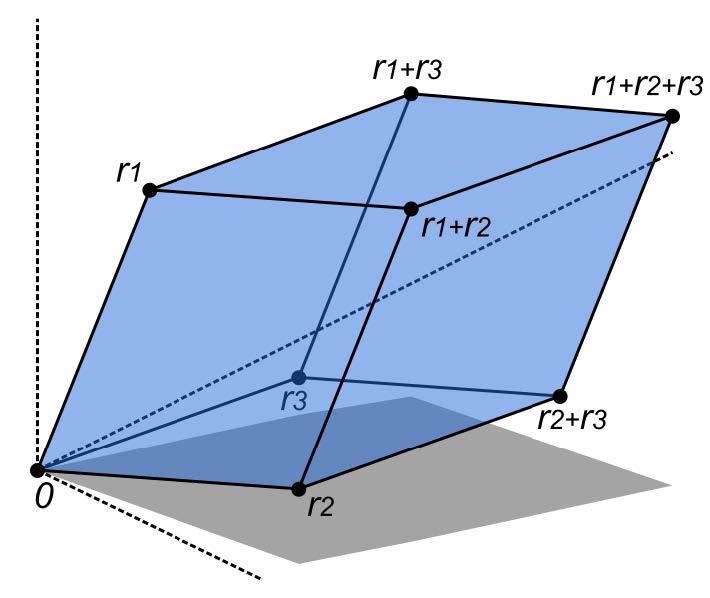
\includegraphics[width=0.35\textwidth]{/Lec1/03}
        \end{figure}
        \item \transtip{特征向量与特征值}{Eigenvectors and Eigenvalues}
        \begin{enumerate}
            \item $Ax=\lambda x$, $A$对特征向量x的变换等价于对x 的缩放, 没改变x的方向
            \item $A=Q\Lambda Q^{-1}$, 直接调用函数实现
            \begin{figure}[H]
                \centering
                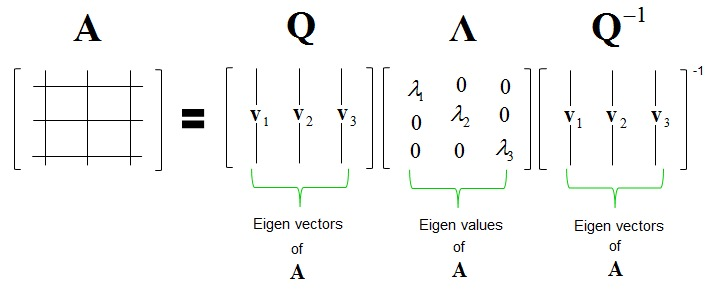
\includegraphics[width=0.35\textwidth]{/Lec1/01}
            \end{figure}
            特征值不一定是实数(可能是复数), 仅$A$为对称时才是实数
            \item 应用: 主成分分析. 一堆点找一个方向, 在这个方向上这些点的方差最大. 
            \begin{figure}[H]
                \centering
                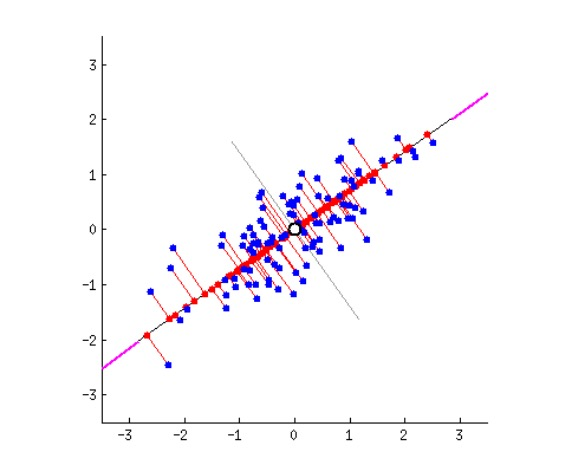
\includegraphics[width=0.35\textwidth]{/Lec1/02}
            \end{figure}
            将点记为$A$, 最大方向就是$A^{-1}A$最大特征值的特征向量
        \end{enumerate}
    \end{enumerate}